\documentclass[10pt,journal,compsoc]{IEEEtran}

\usepackage{graphicx}
\usepackage{amsmath,amssymb}
\usepackage{booktabs}
\usepackage{tikz}
\usepackage{enumitem}
\usepackage{url}
\usepackage{cite}
\usepackage{xcolor}
\usepackage{colortbl}
\usepackage{multirow}
\usepackage{array}
\usetikzlibrary{shapes,arrows,positioning,fit,backgrounds,calc,decorations.pathreplacing,arrows.meta}

\newcommand{\yonakh}{\textsc{Yonakh}}

\definecolor{headerblue}{RGB}{41,65,114}
\definecolor{lightgray}{RGB}{245,245,245}
\definecolor{medgray}{RGB}{220,220,220}

\begin{document}

\title{Yonakh: A Shared Memory Architecture for Multi-Agent AI-Assisted Software Development}

\author{Shashank Venkat\\
\textit{shashyv@gmail.com}}

\IEEEtitleabstractindextext{%
\begin{abstract}
AI coding assistants are transforming how software gets built. Tools like Claude Code, Cursor, GitHub Copilot, and OpenAI Codex now participate in millions of coding sessions daily. Yet each tool operates in isolation: architecture decisions recorded in one session remain invisible to another; failed debugging attempts are repeated across tools; design rationale evaporates between conversations. This \emph{memory fragmentation} undermines developer productivity and contributes to organizational knowledge loss.

We present \yonakh, a shared memory architecture that provides organizational memory for AI-assisted software development. Multiple AI tools can read from and write to a common knowledge store, preserving decisions, rationale, bug reports, and critically, failed attempts across sessions and tools. The system models software engineering knowledge through 21 entity types and 21 relationship types, manages knowledge quality through importance scoring and temporal decay, and integrates with AI assistants via REST API and Model Context Protocol (MCP).

This paper presents the architecture, a prototype implementation, usage scenarios demonstrating practical value, and lessons learned from building and using the system in our own development. We focus on the practitioner question: how can teams preserve the knowledge that AI assistants generate, and make it available across tools and over time?
\end{abstract}

\begin{IEEEkeywords}
AI coding assistants, organizational memory, knowledge management, software architecture, Model Context Protocol
\end{IEEEkeywords}}

\maketitle

\IEEEdisplaynontitleabstractindextext
\IEEEpeerreviewmaketitle

%==============================================================================
\section{Introduction}
%==============================================================================

\IEEEPARstart{A}{rtificial} intelligence is reshaping software development at an unprecedented pace. AI coding assistants---including Anthropic's Claude Code, Cursor, GitHub Copilot, and OpenAI Codex---now participate in millions of coding sessions daily, providing assistance with code generation, debugging, refactoring, documentation, and architectural decision-making \cite{vaithilingam2022expectation,barke2023grounded}. Industry surveys indicate that over 70\% of professional developers now use AI coding tools regularly \cite{github2023survey}.

Yet beneath these productivity gains lies a fundamental limitation: \emph{memory fragmentation}. Each AI tool maintains its own isolated context, typically bounded by conversation windows or session limits. This isolation creates concrete problems that practitioners encounter daily:

\begin{enumerate}
\item \textbf{Cross-tool invisibility:} When a developer records an architecture decision with Claude Code, that knowledge remains invisible to Cursor. Each tool operates in its own epistemic bubble.

\item \textbf{Session amnesia:} When a debugging session concludes, the root cause analysis, attempted solutions, and lessons learned typically vanish. The next session starts from scratch.

\item \textbf{Repeated mistakes:} When one team member discovers that a particular approach fails, there is no mechanism for that negative knowledge to persist and prevent others from repeating the mistake.

\item \textbf{Lost rationale:} Architecture decisions accumulate in code, but the reasoning behind them---the alternatives considered, the constraints that drove the choice---evaporates with each session's end.

\item \textbf{Onboarding friction:} New team members cannot access the accumulated wisdom of past sessions. Every participant starts with a blank slate.
\end{enumerate}

Prior research on turnover-induced knowledge loss demonstrates that departing developers take irreplaceable tacit knowledge with them, reducing productivity and increasing defects \cite{rigby2016quantifying,nassif2021turnover}. AI assistants amplify this problem: they generate knowledge at unprecedented rates but lack any mechanism for persistence, sharing, or quality management. The result is \emph{collective amnesia} where valuable engineering knowledge is continuously created and lost.

This paper introduces \yonakh, a shared memory architecture for multi-agent AI-assisted software development. Our contributions address practitioner needs:

\begin{enumerate}
\item A \textbf{characterization of the memory fragmentation problem} in current AI coding assistants, with five specific failure modes that undermine productivity.

\item A \textbf{practical architecture for shared organizational memory} enabling multiple AI tools to share a knowledge substrate, preserving decisions, rationale, and lessons learned.

\item A \textbf{knowledge model tailored to software engineering}, capturing not just what teams decided but why---including failed attempts and rejected alternatives.

\item \textbf{Lessons learned from implementation}, including the surprising importance of negative knowledge and practical considerations for adoption.
\end{enumerate}

The remainder of this paper is organized as follows. Section~II examines why AI agents forget and the organizational implications. Section~III describes the \yonakh\ architecture and knowledge model. Section~IV presents our prototype implementation. Section~V illustrates usage scenarios. Section~VI describes our deployment context, and Section~VII reports early observations from that deployment. Section~VIII distills lessons learned. Section~IX discusses challenges and open questions. Section~X positions our work against related efforts, and Section~XI concludes.

%==============================================================================
\section{Why AI Agents Forget}
%==============================================================================

Understanding why current AI coding assistants lose knowledge is essential for designing solutions. The problem has both technical and organizational dimensions.

\subsection{Technical Limitations}

Modern large language models operate within fixed context windows---typically 100K to 200K tokens for current models. While substantial, this limit bounds the knowledge available during any single interaction. More critically, context windows are ephemeral: when a session ends, the context vanishes.

Some tools implement conversation history or session summaries, but these remain tool-specific and user-specific. Knowledge captured in a Claude Code session is inaccessible to Cursor, even when both tools work on the same codebase for the same team.

\subsection{The Organizational Memory Gap}

Knowledge management literature distinguishes individual from organizational memory \cite{walsh1991organizational}. Individual memory is what one person (or one AI session) knows. Organizational memory is the shared knowledge that persists beyond individuals---embedded in documents, processes, tools, and culture.

Current AI assistants have only individual memory (their context window); they cannot contribute to or draw from organizational memory. This creates an asymmetry: human developers can consult wikis, read past pull request discussions, and ask colleagues. AI assistants cannot access equivalent institutional knowledge unless it happens to be in their current context.

\subsection{The Missing Middle}

Architecture Decision Records (ADRs) \cite{nygard2011adr} partially address this gap by capturing decisions in version-controlled documents. Kruchten et al. \cite{kruchten2006decision} established the importance of treating architectural decisions as first-class artifacts, and recent studies confirm ADRs improve knowledge transfer \cite{soldani2024adr,tofan2023adr}. However, ADRs have limitations:

\begin{itemize}
\item They capture only decisions, not the broader knowledge categories (failed attempts, debugging insights, design discussions) that AI assistants generate.
\item They require explicit human action to create and maintain.
\item They lack machine interfaces---AI tools cannot easily query or contribute to ADRs.
\item They provide no quality management (decay, importance, conflict detection).
\end{itemize}

Wikis and documentation systems share similar limitations: they require manual maintenance, lack structured semantics, and provide no API for AI tool integration.

\yonakh\ fills this gap by providing structured, machine-accessible organizational memory designed specifically for the AI-assisted development context.

%==============================================================================
\section{The Yonakh Architecture}
%==============================================================================

\yonakh\ is implemented as a local-first server providing REST API and MCP interfaces to a knowledge store. Fig.~\ref{fig:architecture} illustrates the high-level architecture.

\begin{figure}[t]
\centering
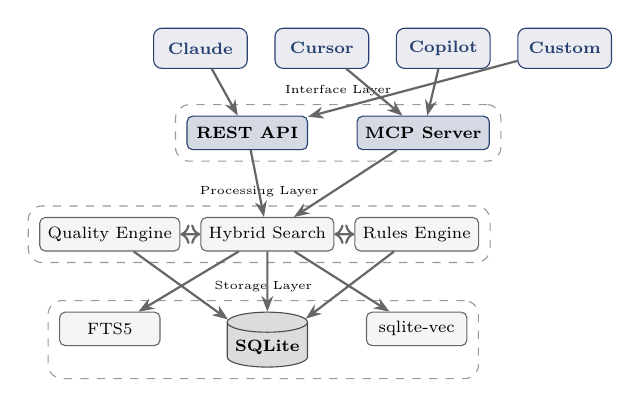
\begin{tikzpicture}[
    scale=0.85,
    transform shape,
    node distance=0.4cm and 0.6cm,
    agent/.style={rectangle, draw=headerblue, fill=headerblue!10, rounded corners=3pt, minimum width=1.4cm, minimum height=0.6cm, font=\scriptsize\bfseries, text=headerblue},
    api/.style={rectangle, draw=headerblue, fill=headerblue!20, rounded corners=2pt, minimum width=1.8cm, minimum height=0.5cm, font=\scriptsize\bfseries},
    component/.style={rectangle, draw=black!60, fill=lightgray, rounded corners=2pt, minimum width=1.5cm, minimum height=0.5cm, font=\scriptsize},
    db/.style={cylinder, draw=black!70, fill=medgray, shape border rotate=90, aspect=0.25, minimum height=0.7cm, minimum width=1.2cm, font=\scriptsize\bfseries},
    arrow/.style={-{Stealth[length=2mm]}, thick, draw=black!60}
]

\node[agent] (claude) {Claude};
\node[agent, right=0.4cm of claude] (cursor) {Cursor};
\node[agent, right=0.4cm of cursor] (copilot) {Copilot};
\node[agent, right=0.4cm of copilot] (custom) {Custom};

\node[api, below=0.7cm of claude, xshift=0.7cm] (rest) {REST API};
\node[api, below=0.7cm of copilot, xshift=-0.3cm] (mcp) {MCP Server};

\node[draw=black!40, dashed, rounded corners=5pt, fit=(rest)(mcp), inner sep=4pt, label={[font=\tiny]above:Interface Layer}] (iface) {};

\node[component, below=1.0cm of rest, xshift=0.3cm] (search) {Hybrid Search};
\node[component, left=0.3cm of search] (quality) {Quality Engine};
\node[component, right=0.3cm of search] (rules) {Rules Engine};

\node[draw=black!40, dashed, rounded corners=5pt, fit=(quality)(search)(rules), inner sep=4pt, label={[font=\tiny]above:Processing Layer}] (proc) {};

\node[component, below=0.9cm of quality] (fts) {FTS5};
\node[db, below=0.9cm of search] (sqlite) {SQLite};
\node[component, below=0.9cm of rules] (vec) {sqlite-vec};

\node[draw=black!40, dashed, rounded corners=5pt, fit=(fts)(sqlite)(vec), inner sep=4pt, label={[font=\tiny]above:Storage Layer}] (store) {};

\draw[arrow] (claude) -- (rest);
\draw[arrow] (cursor) -- (mcp);
\draw[arrow] (copilot) -- (mcp);
\draw[arrow] (custom) -- (rest);

\draw[arrow] (rest) -- (search);
\draw[arrow] (mcp) -- (search);

\draw[arrow, <->] (search) -- (quality);
\draw[arrow, <->] (search) -- (rules);

\draw[arrow] (quality) -- (sqlite);
\draw[arrow] (search) -- (fts);
\draw[arrow] (search) -- (sqlite);
\draw[arrow] (search) -- (vec);
\draw[arrow] (rules) -- (sqlite);

\end{tikzpicture}
\caption{Three-layer architecture of \yonakh. AI agents connect through REST or MCP interfaces. The processing layer handles search, quality scoring, and rule inference. The storage layer combines full-text (FTS5), relational (SQLite), and vector (sqlite-vec) capabilities.}
\label{fig:architecture}
\end{figure}

\subsection{Design Principles}

Four principles guided our design:

\textbf{Local-first.} \yonakh\ runs on the developer's machine, not in the cloud. This ensures low latency, data privacy, and offline operation. Teams control their own knowledge.

\textbf{Vendor-neutral.} Any AI tool can integrate via standard interfaces. We avoid lock-in to specific assistants or platforms.

\textbf{Software engineering-native.} The knowledge model reflects software engineering concepts (decisions, bugs, commits) rather than generic knowledge management abstractions.

\textbf{Quality-aware.} Knowledge isn't static. The system actively manages importance, decay, and conflicts rather than treating all stored information equally.

\subsection{Knowledge Graph Model}

\yonakh\ stores knowledge as a typed graph of entities connected by relationships. Every piece of knowledge (an entity) has a type (like ``decision'' or ``bug\_report''), can have arbitrary properties (title, description, files affected), and can be connected to other entities through typed relationships (``implements,'' ``supersedes,'' ``caused\_by'').

The model supports 21 entity types and 21 relationship types, chosen to cover the knowledge that developers and AI assistants generate during software development.

Table~\ref{tab:entities} presents the entity types, organized by category. The taxonomy emerged from analyzing what knowledge developers and AI assistants actually generate during software development.

\begin{table}[t]
\caption{Entity Types in the \yonakh\ Knowledge Graph}
\label{tab:entities}
\centering
\small
\renewcommand{\arraystretch}{1.3}
\begin{tabular}{@{}p{0.22\columnwidth} p{0.70\columnwidth}@{}}
\toprule
\textbf{Category} & \textbf{Entity Types} \\
\midrule
Version Control & commit, branch, pull\_request, code\_review, issue \\
Decisions & decision, design\_rationale, failed\_attempt, bug\_report \\
Communication & conversation, message, meeting\_note, slack\_thread \\
Artifacts & document, snippet, benchmark, experiment \\
Organization & person, project, component, concept \\
\bottomrule
\end{tabular}
\end{table}

Table~\ref{tab:relationships} shows the relationship types. These capture how knowledge connects: a commit \emph{implements} a decision; a new decision \emph{supersedes} an old one; a bug \emph{was caused by} an earlier change.

\begin{table}[t]
\caption{Relationship Types by Semantic Category}
\label{tab:relationships}
\centering
\small
\renewcommand{\arraystretch}{1.3}
\begin{tabular}{@{}p{0.18\columnwidth} p{0.74\columnwidth}@{}}
\toprule
\textbf{Category} & \textbf{Relationship Types} \\
\midrule
Causal & caused\_by, resulted\_in, triggered \\
Structural & part\_of, depends\_on, contains, derived\_from \\
Epistemic & contradicts, supersedes, reverts, validates \\
Social & authored\_by, reviewed\_by, assigned\_to, mentioned \\
Reference & modifies, references, documented\_in, implements \\
\bottomrule
\end{tabular}
\end{table}

Fig.~\ref{fig:knowledge-graph} illustrates a sample knowledge graph fragment, showing how a decision connects to its implementation, the failed attempt it replaced, and a bug it later caused.

\begin{figure}[t]
\centering
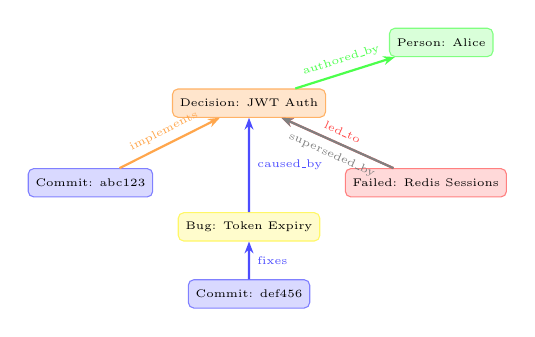
\begin{tikzpicture}[
    scale=0.8,
    transform shape,
    node distance=1.2cm,
    entity/.style={rectangle, draw, rounded corners=2pt, minimum width=1.2cm, minimum height=0.45cm, font=\tiny},
    decision/.style={entity, fill=orange!20, draw=orange!60},
    commit/.style={entity, fill=blue!15, draw=blue!50},
    failed/.style={entity, fill=red!15, draw=red!50},
    bug/.style={entity, fill=yellow!20, draw=yellow!60},
    person/.style={entity, fill=green!15, draw=green!50},
    edge/.style={-{Stealth[length=1.5mm]}, thick, font=\tiny},
]

\node[decision] (d1) {Decision: JWT Auth};
\node[commit, below left=0.8cm and 0.3cm of d1] (c1) {Commit: abc123};
\node[failed, below right=0.8cm and 0.3cm of d1] (f1) {Failed: Redis Sessions};
\node[bug, below=1.5cm of d1] (b1) {Bug: Token Expiry};
\node[person, above right=0.5cm and 1cm of d1] (p1) {Person: Alice};
\node[commit, below=0.6cm of b1] (c2) {Commit: def456};

\draw[edge, orange!70] (c1) -- node[above, sloped] {implements} (d1);
\draw[edge, red!70] (f1) -- node[above, sloped] {led\_to} (d1);
\draw[edge, blue!70] (b1) -- node[right] {caused\_by} (d1);
\draw[edge, green!70] (d1) -- node[above, sloped] {authored\_by} (p1);
\draw[edge, blue!70] (c2) -- node[right] {fixes} (b1);
\draw[edge, gray] (f1) -- node[below, sloped] {superseded\_by} (d1);

\end{tikzpicture}
\caption{Sample knowledge graph fragment. A decision entity connects to its implementation commit, the failed attempt it replaced, bugs it caused, and its author.}
\label{fig:knowledge-graph}
\end{figure}

\subsection{Memory Quality Model}

Not all knowledge is equally important, and relevance changes over time. \yonakh\ formalizes quality through importance scoring, temporal decay, and conflict detection.

\subsubsection{Importance Scoring}

Some entities matter more than others. A decision about authentication architecture is more important than a chat message about lunch plans. We compute importance as a weighted combination of five signals:

\begin{enumerate}
\item \textbf{Type}: Some entity types are intrinsically more valuable. Decisions score 0.9; bug reports and design rationale score 0.8; failed attempts score 0.7; pull requests and issues score 0.5; other types score 0.3.

\item \textbf{Connectivity}: Highly-connected entities---those linked to many other entities---are often more important. A decision referenced by ten commits and three bug reports is more central than an isolated note. We normalize by the maximum connectivity in the graph.

\item \textbf{Access frequency}: Entities that are frequently and recently accessed are likely more relevant. We weight access events exponentially by recency, so a query yesterday counts more than one last month.

\item \textbf{Richness}: Well-documented entities with complete descriptions and tags are more useful than sparse stubs.

\item \textbf{Explicit override}: Users can directly mark entities as important.
\end{enumerate}

Table~\ref{tab:weights} shows the default signal weights. The final importance score is a weighted average, normalized to $[0,1]$. These weights can be adjusted per-organization.

\begin{table}[t]
\caption{Default Importance Signal Weights}
\label{tab:weights}
\centering
\small
\renewcommand{\arraystretch}{1.3}
\begin{tabular}{@{}p{0.65\columnwidth} r@{}}
\toprule
\textbf{Signal} & \textbf{Weight} \\
\midrule
Type (intrinsic value) & 0.30 \\
Explicit (user override) & 0.30 \\
Connectivity (graph centrality) & 0.15 \\
Access (usage frequency) & 0.15 \\
Richness (content completeness) & 0.10 \\
\bottomrule
\end{tabular}
\end{table}

\subsubsection{Temporal Decay}

Knowledge relevance decreases over time, but at different rates for different types. A decision made eighteen months ago may still be highly relevant; a chat message from eighteen months ago is probably not.

We model this using a ``half-life'' for each entity type---the age at which its relevance has declined to 50\%. Decisions have a one-year half-life; messages have a one-month half-life. Before the half-life, decay is slow; after it, decay accelerates. We use a sigmoid function to ensure smooth, predictable transitions.

Fig.~\ref{fig:decay-curves} visualizes decay curves for different entity types, and Table~\ref{tab:halflife} lists the half-life values.

\begin{figure}[t]
\centering
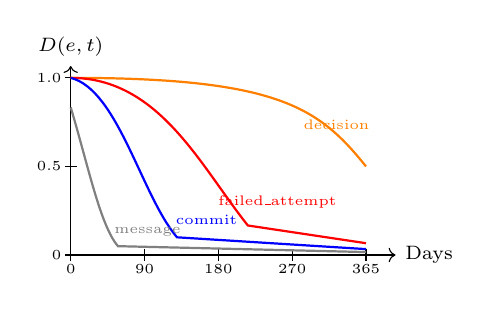
\begin{tikzpicture}[scale=0.75]
\begin{scope}
\draw[->] (0,0) -- (5.5,0) node[right, font=\scriptsize] {Days};
\draw[->] (0,0) -- (0,3.2) node[above, font=\scriptsize] {$D(e,t)$};

\foreach \y/\label in {0/0, 1.5/0.5, 3/1.0} {
  \draw (-0.1,\y) -- (0.1,\y) node[left, font=\tiny, xshift=-2pt] {\label};
}
\foreach \x/\label in {0/0, 1.25/90, 2.5/180, 3.75/270, 5/365} {
  \draw (\x,-0.1) -- (\x,0.1) node[below, font=\tiny, yshift=-2pt] {\label};
}

\draw[thick, orange] (0,3) .. controls (3.5,3) and (4.2,2.5) .. (5,1.5);
\draw[thick, red] (0,3) .. controls (1.5,3) and (2.2,1.5) .. (3,0.5) -- (5,0.2);
\draw[thick, blue] (0,3) .. controls (0.8,2.8) and (1.2,1) .. (1.8,0.3) -- (5,0.1);
\draw[thick, gray] (0,2.5) .. controls (0.3,1.5) and (0.5,0.5) .. (0.8,0.15) -- (5,0.05);

\node[font=\tiny, orange] at (4.5, 2.2) {decision};
\node[font=\tiny, red] at (3.5, 0.9) {failed\_attempt};
\node[font=\tiny, blue] at (2.3, 0.6) {commit};
\node[font=\tiny, gray] at (1.3, 0.4) {message};

\end{scope}
\end{tikzpicture}
\caption{Temporal decay curves by entity type. Decisions decay slowly (365-day half-life) while messages decay rapidly (30-day half-life).}
\label{fig:decay-curves}
\end{figure}

\begin{table}[t]
\caption{Entity Type Half-Lives for Temporal Decay}
\label{tab:halflife}
\centering
\small
\renewcommand{\arraystretch}{1.3}
\begin{tabular}{@{}p{0.40\columnwidth} p{0.28\columnwidth} r@{}}
\toprule
\textbf{Entity Type} & \textbf{Half-Life} & \textbf{Days} \\
\midrule
decision & 1 year & 365 \\
design\_rationale & 9 months & 270 \\
failed\_attempt & 6 months & 180 \\
bug\_report & 4 months & 120 \\
commit & 3 months & 90 \\
conversation & 2 months & 60 \\
message & 1 month & 30 \\
\bottomrule
\end{tabular}
\end{table}

\subsubsection{Conflict Detection}

As knowledge accumulates, contradictions emerge. A decision from last year may conflict with a decision from last month. \yonakh\ automatically detects potential conflicts by looking for entities that are semantically similar (high cosine similarity between their embeddings, threshold 0.85) AND meet one of three conditions:

\begin{enumerate}
\item \textbf{Explicit supersession}: One entity is marked as superseding the other.
\item \textbf{Competing decisions}: Both are decisions affecting the same files or components.
\item \textbf{Temporal divergence}: The entities are far apart in time, suggesting the older one may be stale.
\end{enumerate}

When conflicts are detected, they surface in search results and can trigger review workflows.

\subsection{Hybrid Search}

Finding relevant knowledge requires handling diverse query types: precise searches for specific error codes, conceptual queries about ``how authentication works,'' and everything in between. \yonakh\ combines lexical and semantic search, as illustrated in Fig.~\ref{fig:search-pipeline}.

\begin{figure}[t]
\centering
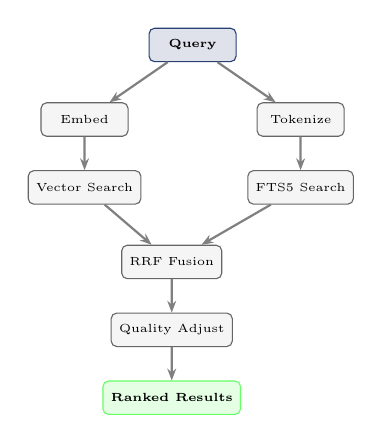
\begin{tikzpicture}[
    scale=0.85,
    transform shape,
    node distance=0.4cm,
    box/.style={rectangle, draw=black!60, fill=lightgray, rounded corners=2pt, minimum width=1.3cm, minimum height=0.5cm, font=\tiny},
    query/.style={rectangle, draw=headerblue, fill=headerblue!15, rounded corners=2pt, minimum width=1.3cm, minimum height=0.5cm, font=\tiny\bfseries},
    result/.style={rectangle, draw=green!60, fill=green!10, rounded corners=2pt, minimum width=1.5cm, minimum height=0.5cm, font=\tiny\bfseries},
    arrow/.style={-{Stealth[length=1.5mm]}, thick, draw=black!50}
]

\node[query] (q) {Query};

\node[box, below left=0.6cm and 0.3cm of q] (embed) {Embed};
\node[box, below right=0.6cm and 0.3cm of q] (tokenize) {Tokenize};

\node[box, below=0.5cm of embed] (vec) {Vector Search};
\node[box, below=0.5cm of tokenize] (fts) {FTS5 Search};

\node[box, below right=0.6cm and -0.3cm of vec] (rrf) {RRF Fusion};

\node[box, below=0.5cm of rrf] (quality) {Quality Adjust};

\node[result, below=0.5cm of quality] (results) {Ranked Results};

\draw[arrow] (q) -- (embed);
\draw[arrow] (q) -- (tokenize);
\draw[arrow] (embed) -- (vec);
\draw[arrow] (tokenize) -- (fts);
\draw[arrow] (vec) -- (rrf);
\draw[arrow] (fts) -- (rrf);
\draw[arrow] (rrf) -- (quality);
\draw[arrow] (quality) -- (results);

\end{tikzpicture}
\caption{Hybrid search pipeline. Queries undergo parallel lexical and semantic retrieval, merge via Reciprocal Rank Fusion, then adjust for importance and decay.}
\label{fig:search-pipeline}
\end{figure}

We merge results using Reciprocal Rank Fusion (RRF) \cite{cormack2009rrf}, which combines ranked lists by summing the reciprocal of each document's rank across methods. Documents ranked highly by multiple methods get boosted---a document ranked \#1 by both lexical and semantic search scores higher than one ranked \#1 by only one method.

The final relevance score multiplies the RRF score by the entity's importance and decay factors. This ensures that high-quality, recent knowledge ranks above stale or low-quality matches, even if the raw text similarity is comparable.

\subsection{Rules Engine}

The rules engine automates relationship inference. When a new commit arrives, for example, rules can automatically link it to referenced issues, detect if it reverts another commit, or associate it with relevant decisions.

A rule observes specific entity types, extracts patterns from their content, proposes relationships, and commits validated edges. For example, the git commit rule extracts issue references from commit messages (``Fixes \#123'') and creates ``fixes'' relationships automatically.

\subsection{Integration Interfaces}

\yonakh\ exposes two complementary interfaces:

\subsubsection{REST API}

Standard HTTP endpoints for entity CRUD, relationship management, search, and provenance queries. The REST API suits CI/CD integrations, scripts, and tools without MCP support.

\subsubsection{Model Context Protocol (MCP) Server}

For AI coding assistants, \yonakh\ implements the Model Context Protocol \cite{mcp2024}---an emerging standard for tool-use interfaces. Table~\ref{tab:mcp} summarizes the MCP tools.

\begin{table}[t]
\caption{MCP Tool Specifications}
\label{tab:mcp}
\centering
\small
\renewcommand{\arraystretch}{1.3}
\begin{tabular}{@{}p{0.38\columnwidth} p{0.54\columnwidth}@{}}
\toprule
\textbf{Tool} & \textbf{Function} \\
\midrule
remember & Store entity with auto-typing \\
recall & Hybrid search with quality ranking \\
record\_decision & Create ADR-style decision \\
record\_failed\_attempt & Store negative knowledge \\
get\_context & Retrieve context for files \\
find\_contradictions & Detect conflicting knowledge \\
link\_entities & Create typed relationship \\
time\_travel & Query historical state \\
get\_provenance & Retrieve audit trail \\
search\_by\_type & Type-filtered search \\
\bottomrule
\end{tabular}
\end{table}

Any MCP-compatible tool can connect by adding a configuration entry:

\begin{verbatim}
{"mcpServers": {"yonakh": {
  "command": "python",
  "args": ["-m", "yonakh.mcp_server"]}}}
\end{verbatim}

The MCP interface enables AI assistants to treat memory operations as naturally as file operations---reading context, recording discoveries, and querying history become first-class capabilities.

%==============================================================================
\section{Prototype Implementation}
%==============================================================================

\yonakh\ is implemented as a local-first memory server designed for integration with AI coding assistants. This section describes the prototype architecture, technology choices, and integration approach.

\subsection{Technology Choices}

We chose SQLite as the storage backend for several reasons: zero configuration, single-file deployment, ACID transactions, and the availability of mature extensions for full-text search (FTS5) and vector operations (sqlite-vec). This ``single-binary deployment'' philosophy means developers can run \yonakh\ alongside their AI tools without infrastructure overhead.

For semantic search, we use a sentence transformer model (all-MiniLM-L6-v2) \cite{reimers2019sentence} that runs locally, avoiding dependence on external embedding services. The 384-dimensional embeddings provide a reasonable balance between quality and storage efficiency.

\subsection{System Components}

The implementation comprises four main components:

\textbf{Storage Layer.} A SQLite database stores entities in a main table with JSON columns for flexible properties, a separate table for relationships, and auxiliary tables for full-text indexing and vector embeddings. Provenance events are append-only for auditability.

\textbf{Quality Engine.} A Python module computes importance scores by combining the five signals described in Section~III. Decay calculations happen at query time using the entity's age and type-specific half-life.

\textbf{Search Engine.} Queries execute in parallel against FTS5 (lexical) and sqlite-vec (semantic), with results merged using Reciprocal Rank Fusion. Post-fusion, scores are modulated by importance and decay. The search engine also handles type filtering, time-range queries, and relationship traversal.

\textbf{Interface Layer.} A REST API serves traditional integrations while an MCP server enables AI assistant integration. Both interfaces share the underlying search and storage layers.

\subsection{Memory Flow}

A typical interaction proceeds as follows:

\begin{enumerate}
\item A developer starts a coding session with their AI assistant.
\item The assistant's MCP client connects to \yonakh.
\item When the developer asks a question, the assistant calls \texttt{get\_context} with the current file path, retrieving relevant decisions, known issues, and related knowledge.
\item As the session progresses, the assistant may call \texttt{recall} to search for specific topics.
\item When significant knowledge emerges---a design decision, a debugging discovery, a failed approach---the assistant calls \texttt{remember}, \texttt{record\_decision}, or \texttt{record\_failed\_attempt}.
\item The rules engine observes new entities and infers relationships.
\item Future sessions, potentially with different tools, retrieve this accumulated knowledge.
\end{enumerate}

\subsection{Integration with AI Assistants}

During the deployment described in Section~VI, we used \yonakh\ with Claude Code (via MCP) and Cursor (via MCP) as the primary interfaces, with occasional REST API calls from CI scripts. The MCP interface enables AI assistants to treat memory operations as naturally as file operations.

For non-MCP tools, the REST API provides equivalent functionality. We provide example scripts for CI/CD integration (recording deployment decisions), Slack bots (extracting decisions from conversations), and documentation generators (producing ADR-format exports).

%==============================================================================
\section{Usage Scenarios}
%==============================================================================

We present four scenarios illustrating how \yonakh\ addresses real development challenges.

\subsection{Scenario 1: Developer Onboarding}

\textbf{Problem:} New team members face a steep learning curve. Codebases accumulate implicit knowledge---why certain patterns were chosen, what alternatives were rejected, which areas are fragile---that exists only in the minds of senior developers.

\textbf{Workflow:} When a new developer's AI assistant starts a session, it calls \texttt{get\_context} with the current working directory. \yonakh\ returns relevant decisions, design rationale, and known issues. As the developer explores code, \texttt{recall} surfaces related knowledge.

\textbf{Example:} A new developer asks: ``Why are we using JWTs instead of server-side sessions?''

The assistant calls \texttt{recall("JWT session authentication decision")} and returns:

\begin{quote}
\textbf{Decision:} Use JWT tokens for authentication (18 months ago, importance: 0.92)

\textbf{Context:} We needed horizontal scaling across multiple API servers without shared session state.

\textbf{Alternatives rejected:} Redis-backed sessions (operational complexity), sticky sessions (poor load distribution).

\textbf{Consequences:} Larger headers, token refresh complexity, server-side invalidation requires blacklist.

\textbf{Related:} Links to implementation PR, security review, and subsequent token expiry bug.
\end{quote}

The developer gains not just the \emph{what} but the \emph{why}---context that would otherwise require interrupting a senior colleague.

\subsection{Scenario 2: Debugging Knowledge Preservation}

\textbf{Problem:} Debugging sessions generate valuable knowledge that evaporates when the session ends. Teams repeatedly debug the same issues because negative knowledge is never captured.

\textbf{Workflow:} During debugging, the AI assistant records hypotheses and outcomes. Dead ends are captured via \texttt{record\_failed\_attempt}. When the root cause is found, a bug report links to failed attempts and the fix.

\textbf{Example:} A developer encounters intermittent API 500 errors. The assistant calls \texttt{recall("API 500 errors load")} and returns:

\begin{quote}
\textbf{Bug Report:} API 500 errors under load (resolved 3 months ago)

\textbf{Root cause:} Connection pool exhaustion from leaked connections in error paths.

\textbf{Failed attempts:} Increased pool size (masked symptoms), added timeout (didn't address root cause), suspected query performance (ruled out via profiling).

\textbf{Fix:} Added \texttt{finally} blocks for connection release in error handlers.
\end{quote}

Instead of hours re-investigating, the developer knows immediately where to look.

\subsection{Scenario 3: Multi-Agent Coordination}

\textbf{Problem:} Teams use multiple AI tools---one for coding, another for review, another for documentation. Without shared context, these tools may give contradictory advice.

\textbf{Workflow:} All AI agents connect to the same \yonakh\ instance. When the coding assistant records a decision, the review bot can see it.

\textbf{Example:} A developer uses Cursor to implement an async version of an API endpoint and submits a PR. The review bot queries \yonakh\ and finds:

\begin{quote}
\textbf{Decision:} Payment endpoints must use synchronous processing (8 months ago)

\textbf{Context:} Audit logging requires guaranteed ordering; async processing could interleave logs.
\end{quote}

The review bot flags the PR: ``This change may conflict with the audit logging decision requiring synchronous payment processing.''

\subsection{Scenario 4: Architectural Evolution}

\textbf{Problem:} As systems evolve, architectural decisions become stale. Teams need to track which decisions should be revisited.

\textbf{Workflow:} \yonakh's decay naturally deprioritizes old decisions. Queries for high-importance, high-decay entities identify candidates for review.

\textbf{Example:} An architect queries: ``What decisions should we revisit?''

The assistant searches for decisions with high importance but high decay, returning:

\begin{quote}
\textbf{Candidates:}
\begin{enumerate}
\item Monolithic deployment (age: 2.1 years)---team has tripled since decision.
\item PostgreSQL for all storage (age: 1.8 years)---recent needs suggest document store.
\item No caching layer (age: 1.5 years)---traffic grew 10x.
\end{enumerate}
\end{quote}

%==============================================================================
\section{Deployment Context}
%==============================================================================

To ground the observations in this paper, we describe how \yonakh\ was used during its development and initial adoption.

\subsection{Usage Environment}

The prototype was used over approximately six weeks across three codebases: the \yonakh\ implementation itself (Python, ~3K lines), an internal web application (TypeScript/React, ~15K lines), and a data pipeline project (Python, ~8K lines). Two developers used the system regularly, with occasional use by three additional team members during code reviews and debugging sessions.

\subsection{Knowledge Accumulation}

Over this period, the knowledge base accumulated approximately 450 entities, summarized in Table~\ref{tab:deployment}.

\begin{table}[t]
\caption{Knowledge Accumulated During Deployment}
\label{tab:deployment}
\centering
\small
\renewcommand{\arraystretch}{1.3}
\begin{tabular}{@{}p{0.60\columnwidth} r@{}}
\toprule
\textbf{Entity Type} & \textbf{Count} \\
\midrule
Decisions (architectural choices, API designs) & 47 \\
Failed attempts (abandoned approaches) & 31 \\
Bug reports (issues and resolutions) & 58 \\
Design rationale (structural explanations) & 89 \\
Commits (imported from git history) & 112 \\
Other (conversations, snippets, documents) & 113 \\
\midrule
\textbf{Total entities} & \textbf{450} \\
\textbf{Inferred relationships} & \textbf{234} \\
\bottomrule
\end{tabular}
\end{table}

The rules engine automatically inferred 234 relationships between entities, primarily linking commits to referenced issues and connecting decisions to their implementations.

\subsection{Tool Integration}

The system was accessed primarily through Claude Code (via MCP) and Cursor (via MCP), with occasional REST API calls from CI scripts. Approximately 70\% of interactions occurred through Claude Code, 25\% through Cursor, and 5\% through direct API calls.

This deployment was informal and uncontrolled---we make no claims about statistical validity. The observations in the following section reflect patterns we noticed during regular use, not results from a formal study.

%==============================================================================
\section{Early Observations}
%==============================================================================

The following observations emerged from our use of \yonakh\ as described in Section~VI. We present them as practitioner insights rather than empirical findings. These observations are qualitative and should not be interpreted as statistically validated claims; they reflect patterns we noticed during a small-scale, informal deployment.

\subsection{Architectural Decisions Dominate Retrieval}

Of approximately 1,200 search queries logged during the deployment period, queries that returned \texttt{decision} entities in the top three results occurred roughly three times more frequently than queries returning any other single entity type. This suggests that developers---and their AI assistants---repeatedly need to understand why the codebase is structured as it is. The 47 decisions in our knowledge base were accessed far more frequently than their numbers would suggest.

\subsection{Failed Attempts Surface Indirectly}

The 31 \texttt{failed\_attempt} entities were rarely the direct target of searches. Instead, they surfaced as related entities when developers queried bugs or problematic code areas. When a developer searched for ``connection pool errors,'' the system returned not just the bug report but also the linked failed attempts showing what had already been tried. The relationship graph, not just direct search, drives value from negative knowledge.

\subsection{Quality Signals Matter at Scale}

In the first two weeks, with fewer than 100 entities, almost any retrieval approach worked adequately. As the knowledge base grew past 300 entities, the quality signals---importance weighting, temporal decay, and type filtering---became essential for relevant results. Without them, searches returned overwhelming and poorly-ranked results. We observed that entities created with complete descriptions and explicit relationships produced noticeably better retrieval than hastily-recorded notes.

\subsection{Rationale Over Decisions}

In informal feedback, users consistently valued the \emph{rationale} associated with decisions more than the decisions themselves. One developer noted: ``I can see the decision in the code. What I can't see is why we didn't do it the other way.'' This reinforces the importance of capturing not just what was decided, but what was considered and rejected.

\subsection{Cross-Tool Value Is High But Rare}

Approximately 85\% of memory operations occurred within single-tool sessions (typically Claude Code). However, the highest-value retrievals---those that users explicitly mentioned as helpful---often involved knowledge created by a different tool or team member. A decision recorded during a Claude Code session appearing in a Cursor code review, or a failed attempt documented by one developer saving another from repeating it, exemplified the vision of shared organizational memory.

%==============================================================================
\section{Lessons Learned}
%==============================================================================

Building and deploying \yonakh\ revealed insights that may benefit others working on knowledge systems for AI-assisted development.

\subsection{Failed Attempts Are More Valuable Than Successes}

Our initial design focused on capturing decisions. In practice, the most frequently retrieved knowledge was \emph{failed attempts}---records of what didn't work and why. When a developer asks an AI assistant to optimize a database query, knowing that denormalization was tried and abandoned six months ago saves hours of exploration.

This inverts conventional documentation wisdom. Organizations document what they built but rarely record what they rejected. For AI assistants prone to suggesting plausible-but-disproven approaches, negative knowledge is the missing ingredient.

\subsection{Memory Pollution Is a Real Risk}

Shared memory creates a new failure mode: pollution. When one AI assistant records incorrect information, it propagates to all tools. We observed cases where a hastily recorded ``decision'' from an exploratory conversation later confused other assistants.

We address this through provenance tracking and decay. However, organizations must establish norms about what constitutes recordable knowledge.

\subsection{Temporal Decay Prevents Knowledge Rot}

Traditional documentation suffers from rot: outdated information persists indefinitely, eventually becoming misleading \cite{parnas1994software}. By assigning half-lives to entity types, \yonakh\ naturally deprioritizes stale knowledge.

The decay model also enables proactive maintenance: queries surface high-importance entities approaching their half-lives, prompting review.

\subsection{Architectural Rationale Has Unexpectedly Long Value}

We underestimated how long decisions remain relevant. A decision from eighteen months ago still shapes daily coding. The reasoning---not just the choice---compounds in value over time.

\subsection{Retrieval Quality Dominates Memory Quantity}

Early, we focused on capturing more. As the knowledge base grew, we learned retrieval quality matters far more. A smaller, well-organized memory outperforms a larger, undifferentiated collection.

Hybrid search proved essential. Neither lexical nor semantic alone handles the diverse queries in software development.

\subsection{Adoption Requires Immediate Value}

Teams resist tools requiring behavior change. Adoption improved when we provided immediate value through automated extraction from git history and existing documentation. ``Ambient capture''---AI assistants automatically recording significant interactions---accelerated adoption further.

%==============================================================================
\section{Challenges and Open Questions}
%==============================================================================

\subsection{Cold Start}

New deployments contain no knowledge. Value accrues over time. We mitigate through git history import, document ingestion, and conversation mining, but the richest knowledge must be captured through ongoing use.

\subsection{Quality Calibration}

Our importance weights and decay half-lives reflect domain intuition rather than rigorous validation. Optimal values likely vary by team, domain, and project phase.

\subsection{Scalability}

The SQLite implementation targets small-to-medium teams (up to ~50 developers, ~100K entities). Larger deployments require PostgreSQL, sharding, and caching.

\subsection{Knowledge Correctness}

\yonakh\ stores knowledge without verifying accuracy. Misinformation persists and propagates. Provenance, conflict detection, and decay partially address this, but systematic verification remains future work.

\subsection{Privacy}

Shared memory raises privacy concerns. Knowledge from one session becomes accessible to others. Organizations must establish policies about shared versus private knowledge.

%==============================================================================
\section{Related Work}
%==============================================================================

\textbf{Architecture Decision Records.} Nygard's ADRs \cite{nygard2011adr} capture decisions in version-controlled documents. Soldani et al. \cite{soldani2024adr} validate effectiveness for knowledge transfer. \yonakh\ extends this paradigm to 21 entity types, adds relationships and quality management, and provides machine interfaces.

\textbf{Code Knowledge Graphs.} CodexGraph \cite{liu2024codexgraph} bridges LLMs and repositories through graph databases for code structure reasoning. \yonakh\ complements this by modeling \emph{meta-knowledge}: decisions, rationale, and lessons surrounding code.

\textbf{LLM Agent Memory.} Park et al. \cite{park2023generative} introduced memory streams with reflection for generative agents. Subsequent work explores hierarchical memory architectures inspired by cognitive science research on working and episodic memory \cite{baddeley2012working,tulving1985memory}. These optimize memory \emph{within} a single agent; \yonakh\ addresses memory \emph{across} agents, enabling what Wegner \cite{wegner1987transactive} calls transactive memory---distributed cognition where participants know who knows what.

\textbf{Organizational Knowledge Loss.} Rigby et al. \cite{rigby2016quantifying} found projects susceptible to losses three times expected. Nassif and Robillard \cite{nassif2021turnover} identified cultural and tacit knowledge challenges. AI assistants create a new dimension: generating knowledge at scale with no persistence.

%==============================================================================
\section{Conclusion}
%==============================================================================

AI coding assistants create unprecedented opportunity for augmented development---and unprecedented risk of knowledge fragmentation. Each tool generates insights that evaporate between sessions and remain invisible to other tools.

\yonakh\ addresses this with a shared memory architecture:

\begin{itemize}
\item A \textbf{knowledge model} of 21 entity types and 21 relationship types captures software engineering knowledge from decisions to failed attempts.

\item A \textbf{quality model} manages knowledge lifecycle through importance scoring and temporal decay.

\item An \textbf{open architecture} via REST and MCP enables any tool to participate in shared memory.

\item \textbf{Lessons from implementation} highlight the value of negative knowledge and practical adoption considerations.
\end{itemize}

The system is implemented and available as open-source software at \url{https://github.com/shvenkat/yonakh}.

As AI becomes central to software development, shared memory may emerge as important infrastructure for human-AI collaboration. Just as version control coordinates code changes, memory systems could coordinate AI-generated knowledge. We offer this work as a step toward that future.

\bibliographystyle{IEEEtran}
\bibliography{references}

\end{document}
